\documentclass[fleqn,11pt]{paper}
\usepackage[utf8]{inputenc}
\usepackage[T1]{fontenc}
\usepackage{apacite}
\renewcommand{\doiprefix}{}
\newcommand{\doi}[1]{https://doi.org/#1}

\title{Physiological sensor based mental workload assessment: A multimodal deep learning approach}

\author[1]{Bart-Jan Boverhof \thanks{b.boverhof@students.uu.nl}}
\affil[1]{\normalsize Faculty of Social and Behavioural Sciences, Utrecht University}


\begin{abstract}
The approach of using physiological sensors for the assessment of mental workload has gained in popularity in recent years. We utilized three physiological sensors in predicting mental workload, being electroencephalography (EEG), photoplethysmography (PPG) and galvanic skin response (GSR). Deep learning poses a promising, yet novel, approach towards the modeling of such sensory data. Four deep neural network architectures were created and contrasted in their performance. Three out of four were specified to predict workload based on on a single of the aforementioned physiological sensors, whilst the fourth architecture was a joint neural network combining all physiological signals into a single model. In this study we investigated 1) which physiological sensor individually constitutes the most adequate predictor of mental workload, and 2) whether an approach utilizing multiple sensors simultaneously (i.e. multimodal) is preferable over the approaches utilizing just one. Altogether the EEG-only architecture was found to perform best displaying a mean absolute error of 0.110. We thus conclude that EEG may be considered the most adequate predictor of workload. A mean absolute error of 0.119 was found for the GSR-only architecture. Against expectations, the multimodal approach was outperformed by both aforementioned architectures, displaying a mean absolute error of 0.128. The PPG-only architecture was found to perform worst, displaying a mean absolute error of 0.136. We posed several explanations that help rationalize why the multimodal architecture was found to perform suboptimal, one being an imperfect model architecture, and another being overfitting as resulting from a limited amount of data. Regardless, we demonstrated that the differences in performance across the four network architectures were rather small, i.e. all four neural network architectures performed adequately. 
\end{abstract}

\begin{document}
\begin{titlepage}
\vspace{10mm}

\begin{Large}
{\setlength{\parindent}{0cm}
Methodology and Statistics for the Behavioural, Biomedical and Social Sciences
}
\vspace{2mm}
\newline Utrecht University, the Netherlands
\vspace{18mm}
\newline MSc Thesis Bart-Jan Boverhof (6000142)
\vspace{2mm}
\newline Physiological sensor based prediction of mental workload: A multimodal deep learning approach
\vspace{2mm}
\newline May 2021
\vspace{18mm}
\newline Supervisor:
\vspace{1mm}
\newline Prof. Dr. Ir. Bernard Veldkamp
\vspace{10mm}
\newline Second grader:
\vspace{1mm}
\newline Prof. Dr. Ir René Eijkemans
\vspace{10mm}
\newline Preferred journal of publication: Frontiers in Neuroscience
\vspace{1mm}
\newline Word count: 5603
\end{Large}
\end{titlepage}

\flushbottom
\maketitle
% * <john.hammersley@gmail.com> 2015-02-09T12:07:31.197Z:
%
%  Click the title above to edit the author information and abstract
%
\thispagestyle{empty}

\section{Introduction}
The topic of mental workload is a widely studied phenomenon across a variety of different fields, amongst others the field of ergonomics \cite{young2015state}, human factors \cite{pretorius2007development} and cognitive neurosciences \cite{shuggi2017mental}. A commonly utilized definition of mental workload, hereafter referred to as simply "workload", is the demand placed upon one whilst carrying out a particular task. As rightfully pointed out by \citeA{de1996measurement}, the aforementioned definition is incomplete, for it defines workload solely as a phenomenon external to the individual. Workload, however, requires to be recognized as a person-specific construct, for the amount of perceived workload ushered by a given task may vary substantially between individuals \cite{de1996measurement}. 

A commonly employed method for the assessment of workload in an experimental setting is the well established NASA-Task Load Index questionnaire, hereafter referred to as \enquote{NASA-TLX}. This method embodies several dimensions, jointly inquiring into the amount of perceived workload \cite{hart2006nasa}. Recently, a novel approach has gained in popularity, however. This promising approach constitutes the use of physiological sensors, worn throughout the entire duration of the experiment. The advantage of this approach, is that the development of perceived workload may be monitored throughout the entire experiment, enabling the possibility to precisely monitor the impact of a specific task on a participant's level of workload. Another advantage is that the method may be personalized, which could simply be done by creating and training an individual model for each participant. By doing this, the person-specific character that is inherent to workload is acknowledged, the importance of which was stressed in the opening paragraph of this paper. 

With the current research we explore the feasibility of an approach towards workload assessment by means of various physiological sensors, hereafter referred to as \enquote{modalities}. The three utilized modalities are electroencephalography (EEG), photoplethysmography (PPG) and galvanic skin response (GSR). EEG is a technique that monitors electrical activity in the brain, and is often utilized in the assessment of workload \cite{berka2005evaluation, craik2019deep, hogervorst2014combining}. GSR is a technique that measures electrical conductance of the skin, and equally so is a widely adopted approach to workload assessment \cite{nourbakhsh2012using, zhou2015dynamic}. Lastly, also heart-rate is a widely utilized indicator of workload, mostly obtained through PPG \cite{zhang2018evaluating,jimenez2018using}. 

In this project we opted for a deep learning approach towards modeling. A range of four different deep neural network architectures, hereafter referred to as \enquote{DNN's} or simply \enquote{networks},  are constructed and contrasted in their performance. Among these are three unimodal DNN architectures, each utilizing only a single modality. Thus,  one architecture solely utilizes the EEG modality,  one solely utilizes the GSR modality and one solely utilizes the PPG modality. The fourth is a multimodal architecture, combining all three aforementioned modalities into a single framework. The main advantage of taking a deep learning approach resides its flexibility: designing a network architecture that combines multiple modalities may be done in a relatively straightforward manner \cite{ramachandram2017deep}. 

With this research we 1) seek to explore which individual modality constitutes the most adequate predictor of workload when taking a deep learning approach, and 2) whether a multimodal DNN architecture is preferable over the three simpler (but much less computationally demanding) unimodal network architectures. With regards to the first point, only a single study was found that contrasted several modalities in their ability to predict workload. \citeA{hogervorst2014combining} contrasted multiple modalities, and reported EEG to be the best performing.We therefore carefully hypothesize the EEG modality to be the most adequate predictor of workload. With regards to the second point, we expect the multimodal approach to attain better performance as compared with the unimodal approaches, for predictions are based on richer composite of information. This expectation is indeed in line with previous research, which reported a multimodal approach to perform superiorly \cite{dolmans2020perceived, han2020classification,rastgoo2019automatic, yin2017recognition}. Taking a deep learning approach such as ours may still be considered a novel, yet promising, approach to workload assessment. Due to the novelty of this approach, a deepening of the body of knowledge is necessary, which is something we aim to contribute to with this study.

%Method section
\vspace{10mm}
\section{Data \& Methods}
\subsection{Related Work} \label{sec:related}
The following section provides an overview of preceding research on the assessment of workload by means of various physiological sensors, with a focus on deep learning approaches. Attention is predominantly placed upon network architectures and hyperparameter optimization. In this section we will solely describe previous work: an in depth description of our adopted modeling approach follows in Section \ref{section:DNN}.

\subsubsection*{EEG Network Architecture}
An overview of the complete literature on EEG applications with deep learning was presented by \citeA{craik2019deep}, who reported 16\% of all publications to constitute workload assessment. \citeA{tabar2016novel} proposed a ConvNet and stacked auto-encoder (SAE) hybrid approach towards workload classification with EEG. Their proposed network constituted two different parts. Firstly, raw EEG data was fed into a single convolutional layer, with the objective of extracting features. Secondly, the extracted features were fed into the SAE part of the network,  which encompassed a stack of dense-layers designed to ultimately result in a classification of workload.  An accuracy of 90\% was acquired with this architecture \cite{tabar2016novel}. A similar approach was proposed by \citeA{schirrmeister2017deep}, who contrasted different DNN architectures in their ability to adequately decode EEG signals. Several ConvNet architectures were contrasted against the baseline method for EEG decoding, filter bank common spatial pattern (FBCSP). A deep ConvNet, a shallow ConvNet, a deep-shallow hybrid ConvNet and a residual ConvNet were contrasted with the FBCSP baseline method. Both the deep and shallow ConvNets were found to reach at least similar, and in some regards better, classification results as compared with the FBCSP baseline approach. Altogether, a deep ConvNet with four convolutional-max-pooling blocks was found to perform best, exhibiting a classification accuracy of 92.4\% \cite{schirrmeister2017deep}.

\subsubsection*{GSR Network Architecture}
\citeA{sun2019hybrid} explored various deep-learning approaches towards the classification of emotional states with GSR. Despite that this application differs from workload prediction, inspiration may still be drawn from their utilized architecture. Various models were explored, amongst others a support vector machine, a ConvNet and a long-short-term-memory (LSTM) network. In addition to these, a hybrid ConvNet-LSTM approach was explored as well. This hybrid approach constituted four convolutional blocks, followed by a single LSTM layer, and was found to perform best with an accuracy of 74\% \cite{sun2019hybrid}. \citeA{dolmans2020perceived} contrasted several physiological signals in their ability to predict workload, each of which by taking a deep learning approach. One of these modalities constituted GSR, for which a ConvNet-LSTM hybrid network architecture was utilized to predict workload. The performance of this DNN was contrasted with a network consisting solely of fully connected dense layers. Conform with the previously mentioned findings by  \citeA{sun2019hybrid}, the ConvNet-LSTM hybrid architecture was found to perform best, displaying an absolute difference between predicted and true label of 0.180 (scaled on 0-1). This network architecture incorporated two convolutional blocks, followed by two LSTM layers \cite{dolmans2020perceived}.

\subsubsection*{PPG Network Architecture}
Research by \citeA{biswas2019cornet} explored a PPG deep learning approach, in which their objective was to perform both bio-metric identification and obtain heart rate information. Again, despite that this research doesn't constitute workload prediction or classification, inspiration may still be drawn from the employed network architecture. An exceptional performance of 96\% accuracy was realized with a ConvNet-LSTM hybrid, incorporating two convolutional max-pooling blocks followed by two LSTM layers \cite{biswas2019cornet}. \citeA{dolmans2020perceived} also explored a deep-learning PPG approach to workload prediction.  A ConvNet constituting two convolutional blocks was found to perform best out of all contrasted PPG architectures, displaying an absolute difference between predicted and true label of 0.1969 (scaled on 0-1).

\subsubsection*{Multimodal Fusion Strategy}  
When creating a DNN that combines multiple modalities into a single architecture,  the information streams that stem from the different subparts of the network (each corresponding to one of the modalities) are required to be combined, i.e. \enquote{fused}, at a given point in the network. This is necessary in order to ultimately end up with a single prediction of workload. Fusion can be done conforming several strategies, out of which three strategies as proposed by \citeA{ramachandram2017deep} are considered.

Firstly, early fusion constitutes an approach that fuses data sources before being fed into the network. Early fusing usually proves to be quite challenging, residing in the fact that data streams stemming from different modalities often differ in their dimensionality and sampling rate. In addition, when taking an early fusion approach, the assumption of conditional independence is made implicitly. This assumption is oftentimes unrealistic in practice, for data stemming from different modalities are expected to be correlated \cite{ramachandram2017deep}. Secondly, late fusion refers to the process of aggregating the decisions of multiple separate networks, each constructed for every modality separately. When the data sources stemming from the various modalities happen to be either correlated, or different in dimensionality, late fusion is oftentimes a more feasible approach as opposed to early fusion \cite{ramachandram2017deep}. Lastly, intermediate fusion is the most widely employed fusion strategy for multimodal networks. Data streams are usually fused by a concatenation layer, joining the outputs of the separately defined network parts of each modality. This results in a single joint deep neural network. Several higher-order layers are usually defined in between the concatenation layer and the ultimate prediction layer. The depth of the fusion, i.e. the specified number of higher-order layers, may be chosen by the researcher, posing intermediate fusion to be the most flexible and therefore the most widely adopted fusion strategy \cite{ramachandram2017deep}.

Indeed when consulting the literature, it becomes apparent that intermediate fusion is the most prevailing strategy for multimodal DNN architectures. As mentioned before, when taking an intermediate fusion approach, the higher-order part of the network is required to be designed by the researcher. \citeA{rastgoo2019automatic} utilized a multimodal ConvNet approach, and fused the modalities by concatenation, followed with two LTSM layers and two dense layers. A simpler approach is adopted by \citeA{han2020classification}, who utilized an intermediate fusion approach solely consisting of several fully connected dense layers. Lastly, \citeA{dolmans2020perceived} took a relatively deep intermediate fusion approach, consisting of two dense layers, two convolutional layers followed by another two dense layers.  

\subsubsection*{Auxiliary Layers in a DNN Architecture}
At the core of a DNN are the previously mentioned types of layers, such as convolutional, LSTM and dense layers. Such layers are oftentimes accompanied with auxiliary layers. The first type of layers often used in network architectures are batch normalization layers, which have the objective of improving network stability. It is beneficial to incorporate a batch normalization layer subsequent to a convolutional layer, but before feeding into the activation layer \cite{ioffe2015batch}.  For a deep dive into batch normalization, we refer the reader to \citeA{ioffe2015batch}. All previously considered network architectures made use of batch normalization layers \cite{biswas2019cornet, dolmans2020perceived, schirrmeister2017deep, sun2019hybrid, tabar2016novel}.

Pooling layers are commonly employed in ConvNets, usually succeeding a convolutional layer with the purpose of reducing dimensionality. The objective of such layers are to down-sample features into a more compact space, hereby only retaining essential information, and thus omitting redundant information. For a more extensive elaboration on pooling we refer the reader to \citeA{lecun2015deep}. All previously considered network architectures utilized max-pooling layers, usually specified subsequent to the activation layer \cite{biswas2019cornet, dolmans2020perceived, schirrmeister2017deep, sun2019hybrid, tabar2016novel}.

The incorporation of dropout was initially proposed by \citeA{srivastava2014dropout}. Dropout layers drop a randomly-selected number of neurons and their connections throughout the training process. More specifically, within each full training run through the data, i.e. each \enquote{epoch}, a different randomly selected set of neurons are fixed to be inactive. Doing so helps to reduce overfitting, particularly for complex network architectures \cite{srivastava2014dropout}.  Most of the previously considered network architectures made use of dropout layers \cite{biswas2019cornet, dolmans2020perceived, schirrmeister2017deep, sun2019hybrid}.

\subsubsection*{Hyperparameter Optimization}
Hyperparameter optimization (HPO) is a technique that can optimize various DNN hyperparameters, such as for example learning rate and dropout rate. Substantial advancements in DNN performance have been attained by utilizing HPO, especially in the case of ConvNets \cite{bergstra2012random}. In theory, one could optimize the entire DNN architecture, including the amount of neurons/filters in dense/convolutional layers, the number of layers in general, whether to use certain layers, etc. There is, however, a strong relationship between the amount of parameters to be optimized and the computational resources required to do so: optimizing many hyperparameters will inflate computational costs substantially. The Optuna toolbox provides a method for creating a parameter search space, out of which values for the hyperparameters may be sampled \cite{akiba2019optuna}. 

\subsection{Data} \label{sec:data}
The subsequent section provides a description of the utilized data and its collection process. Attention is placed upon the experimental setup, the description of the respondents, the utilized devices for data collection, the synchronization process and the data preprocessing approach. 

\subsubsection*{Experimental Setup \& Data Labeling Strategy}
The experimental setting in which our data was collected is the open-source spaceship video-game Empty Epsilon, in which partakers carried out tasks on a virtual spaceship bridge \cite{daid2016empty}. This experiment was instituted by the Brain Computer Interfaces Testbed\footnote{https://bmslab.utwente.nl/} hosted by the University of Twente and carried out in cooperation with Thales Group Hengelo, the Netherlands\footnote{https://www.thalesgroup.com/en/countries/europe/netherlands}. The experiment constituted 15 tasks, differing in difficulty and hence designed to evoke varying degrees of workload. The total duration of the experiment was roughly three hours.  

Respondents were asked to fill out the NASA-TLX questionnaire after each of the 15 task, inquiring into the amount workload perceived during the respective task. Each questionnaire consisted out of six items. The mean of a subset of four of these items were utilized for labeling of the data. Two items were not incorporated into the scale, for they inquired into the perceived physical demands. Since the experiment took place on a computer whilst participants sat behind a desk, we chose to not incorporate such items. Each item, and hence the newly constructed scale, ranges from 0-20, wherein 0 reflects the lowest possible level of workload and 20 reflects the highest possible level of workload.  In order to encourage numerical stability, label scores were normalized to reside in-between 0-1. 

\subsubsection*{Participants}
After having to omit seven participants due to hardware failure, 27 respondents remained in the final analysis.  18 participants were female whereas nine were male. The average age and its standard deviation were $\mu =26$ and $\sigma = 10.31$ respectively. The participants were students recruited from the University of Twente situated in the Netherlands, as well as several employees of Thales Group Hengelo, equally so situated in the Netherlands. 

\subsubsection*{Devices and Synchronization}
The Shimmer3 GSR+ sensor was used for both PPG and GSR measurements. This device was worn on the wrist, whilst signals were communicated wirelessly via Bluetooth. An ear-clip was utilized for measuring PPG, which was automatically converted to heart-rate. Skin conductivity, or GSR, was measured by two electrodes attached to the fingers. EEG measurement was conducted with the Muse 2 multi-sensor headband, equally so whilst communicating signals wirelessly via Bluetooth. The Shimmer3 GSR+ measured on a sampling rate of 256 Hz, whereas the Muse 2 measured at a sampling rate of 220 Hz. 

Given that multiple devices were utilized, data streams were required to be properly synchronized. This was accomplished by means of an application called Lab-Streaming Layer, hereafter referred to as "LSL", developed by \citeA{kothe2018lab}. The three data streams stemming from the two devices were all streamed to LSL during the experiment. LSL subsequently properly synchronizes all data streams in real-time,  such that they are parallel, hence all referring to equivalent points in time. 

\subsubsection*{Data Preprocessing \& Partitioning}
For each participant, the EEG, PPG and GSR data streams were cut into windows of eight seconds, resulting in an average of roughly 351 windows per respondent. 80\% of the windows have been used for training, 10\% for validation within the training process and 10\% for testing final network performance. The partitioning of the windows into training, validation and testing sets was done systematically by selecting every \textit{n-th} window, such that windows over the entire duration of the experiment were represented equally in each partition.  Exactly the same partitions were utilized in the training, validation and testing procedure across the four architectures, in order to ensure a fair comparison.

\subsection{Network Architectures \& Training} \label{section:DNN}
As was shortly elaborated on in the introduction, an advantage of our approach is that an individual network may be trained for every participant separately.  This is helpful, since individuals tend to respond differently towards high workload situations: for some, workload manifests itself mostly through an increase in heart rate detected through PPG, whereas for others, it mainly manifests as an increase in skin conductivity detected through GSR. Since a total of four architectures are contrasted for 27 participants, this resulted in a total of 108 trained networks. Equally so, HPO was conducted for each person individually, resulting in 108 sets of optimized hyperparameters. All networks were constructed in Python, by utilizing the deep-learning toolbox PyTorch \cite{paszke2017automatic}. 

\subsubsection*{Unimodal Network Architectures}
All unimodal architectures drew inspiration from aforementioned research \cite{biswas2019cornet, dolmans2020perceived, schirrmeister2017deep, sun2019hybrid}. We opted for a ConvNet architecture for all three unimodal approaches.

The three unimodal DNN architectures are depicted alongside one another in Figure \ref{fig:singlearchitecture}. Each of the unimodal networks may be distinguished by two separate parts, being the convolutional part and the prediction part.  The objective of the convolutional part is to extract features from the data, and consists of four convolutional blocks. Each convolutional block consists of a convolutional layer, a batch normalization layer, the Exponential Linear Unit (ELU) activation function, and a max-pooling layer respectively. The objective of the prediction part is to predict the amount of perceived workload,  i.e. ultimately resulting in a single prediction of the label. The prediction part constitutes a flatten-layer,  with the objective of representing all input into one dimensional shape, followed by a dropout layer, a dense layer, a Rectified Linear (RELU) activation function, closed by another dense layer. An overview of the amount of utilized filters / neurons for each layer of each architecture is provided in Table \ref{table:modelvariations}. 

\vspace{7mm}
\begin{figure}[h]
\centering
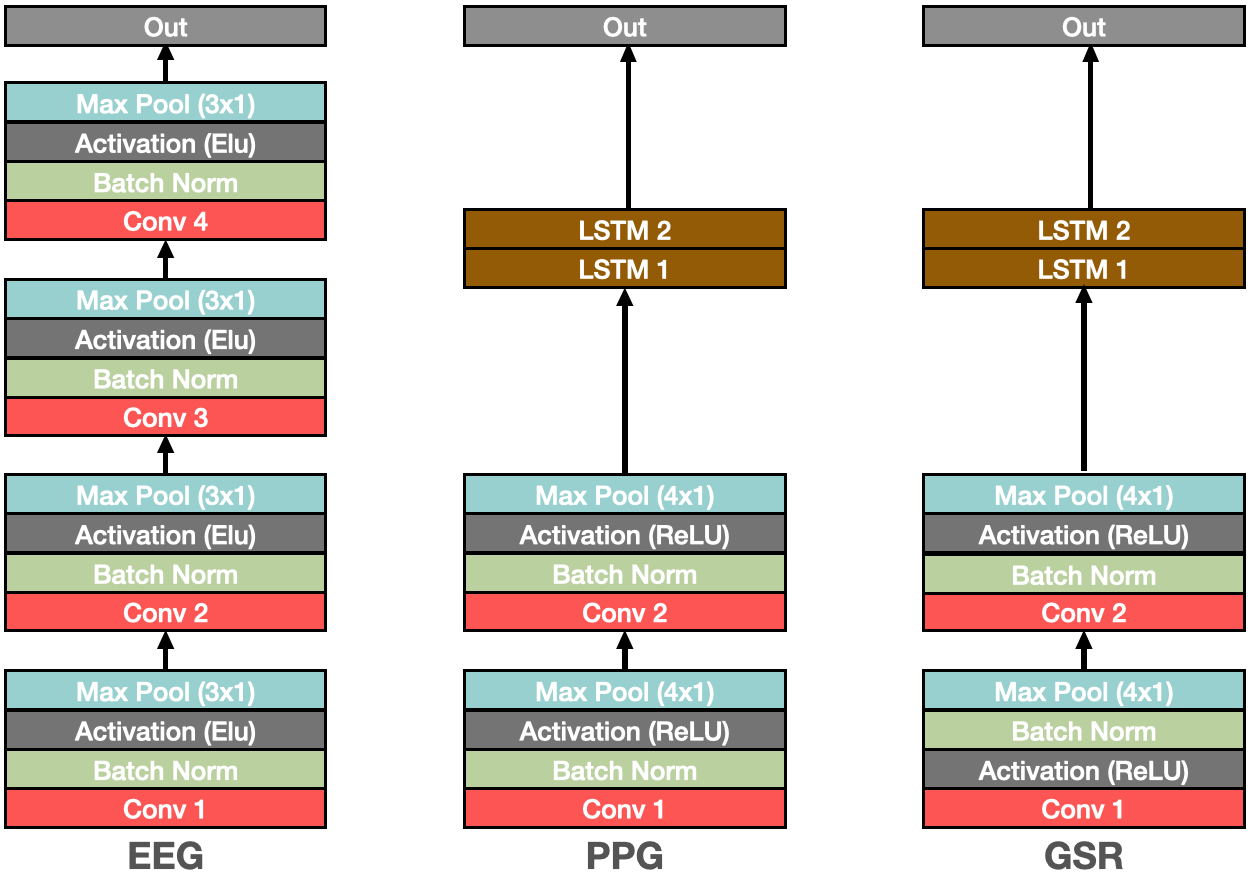
\includegraphics[scale=0.50]{single_model_architecture}
\caption{Unimodal network architectures. Each network architecture constitutes a convolutional part of four convolutional blocks, and a classification part of two fully connected dense layers. }\label{fig:singlearchitecture}
\end{figure}

\newpage
We optimized the hyperparamaters learning rate, dropout rate and the amount of neurons for the first dense layer (\enquote{Dense1} in Figure \ref{fig:singlearchitecture}). This was managed in a total of 50 trials per network.  With respect to network training, a total of 600 epochs have been made through the data for each network specifically. All HPO and training of the unimodal networks was done on a V100 GPU,  offered by the GPU cloud service Google Collab.  Total running time for the unimodal networks was about 96 hours, the most of which was absorbed by HPO. 

\vspace{7mm}
\bgroup
\def\arraystretch{1.4}  
\begin{table}[h]
\begin{center}
\caption{Amount of neurons and filters that each respective layer outputs. }
\label{table:modelvariations}
\begin{tabular}{lllll}
\hline
        & EEG-Net/Part  & GSR-Net/Part  & PPG-Net/Part  & Multimodal Head-Net     \\ \hline
 Unimodal-Nets & Dense Out: 1 & Dense Out: 1 & Dense Out: 1 &   \\
        & Dense 1: \emph{hpo} & Dense1: \emph{hpo} & Dense1: \emph{hpo} &   \\
        \vspace{1.5ex}        
        & Dropout: \emph{hpo} & Dropout: \emph{hpo} & Dropout: \emph{hpo} &   \\
        & Conv4: 200 & Conv4: 128 & Conv4: 128 &    \\ 
        & Conv3: 100 & Conv3: 64 & Conv3: 64 &    \\ 
        & Conv2 50 & Conv2: 32 & Conv2: 32 &    \\ 
        \vspace{1mm}
        & Conv1: 25 & Conv1: 16 & Conv1: 16 &  \\      \hline      
  Multimodal-Net & Dense EEG1: \emph{input} & Dense PPG1: \emph{input} & Dense GSR1: \emph{input} & Dense Out: 1  \\
        & Conv EEG4: 200 & Conv PPG4: 128 & Conv GSR4: 128  &  Dense3: \emph{hpo} \\ 
        & Conv EEG3: 100 & Conv PPG3: 64 & Conv GSR3: 64 & Dense2: \emph{hpo}  \\ 
        & Conv EEG2 50 & Conv PPG2: 32 & Conv GSR2: 32 & Dropout: \emph{hpo}    \\ 
        & Conv EEG1: 25 & Conv PPG1: 16 & Conv GSR1: 16 &    \\   \hline
\end{tabular}
\end{center}
\raggedright \emph{ \newline For all convolutional layers, the depicted numbers reflect the amount of filters that are outputted by the respective layer, whereas for dense layers it reflects the amount of nodes outputted by the respective layer.\textit{\enquote{Input}} refers layers wherein the number of outputting nodes equals the number of inputting nodes.} \par
\end{table}

\subsubsection*{Multimodal Network Architectures} \label{section:multimodal}
The multimodal network architecture was designed by combining the previously characterized unimodal architectures into a single architecture. These separate network parts were joined by a head-network, the architecture of which drew inspiration from aforementioned research by \citeA{han2020classification}. A visual representation of the multimodal network is depicted in Figure \ref{fig:multiarchitecture}. An overview of the amount of utilized filters and neurons per layer is provided in Table \ref{table:modelvariations}.

The feature extraction part of the multimodal network architecture is highly similar to the separate unimodel architectures. We opted for an intermediate fusion strategy, due to its highly flexible nature as compared with alternative fusion strategies (See: Section \ref{sec:related}). The outputs of the three distinct subparts were flattened, followed by a dense layer and RELU activation funtion. Flattening was necessary such that all inputs were represented into one-dimensional space, after which concatenation becomes possible. The prediction part, also referred to as "head-network", consists of three dense layers, alternated with a dropout layer, batch normalization layers and RELU activation layers.  

We optimized the hyperparameters learning rate, dropout rate and the amount of neurons for the first and second dense layers in 18 trials per network.  For training, a total of 250 epochs have been made through the data for each network independently. All training and HPO has been done on a Cloud TPU v2,  offered by the GPU cloud service Google Collab Pro.  Total running time for the multimodal networks was about 120 hours, the most of which absorbed by HPO. 

\vspace{6mm}
\begin{figure}[h]
\centering
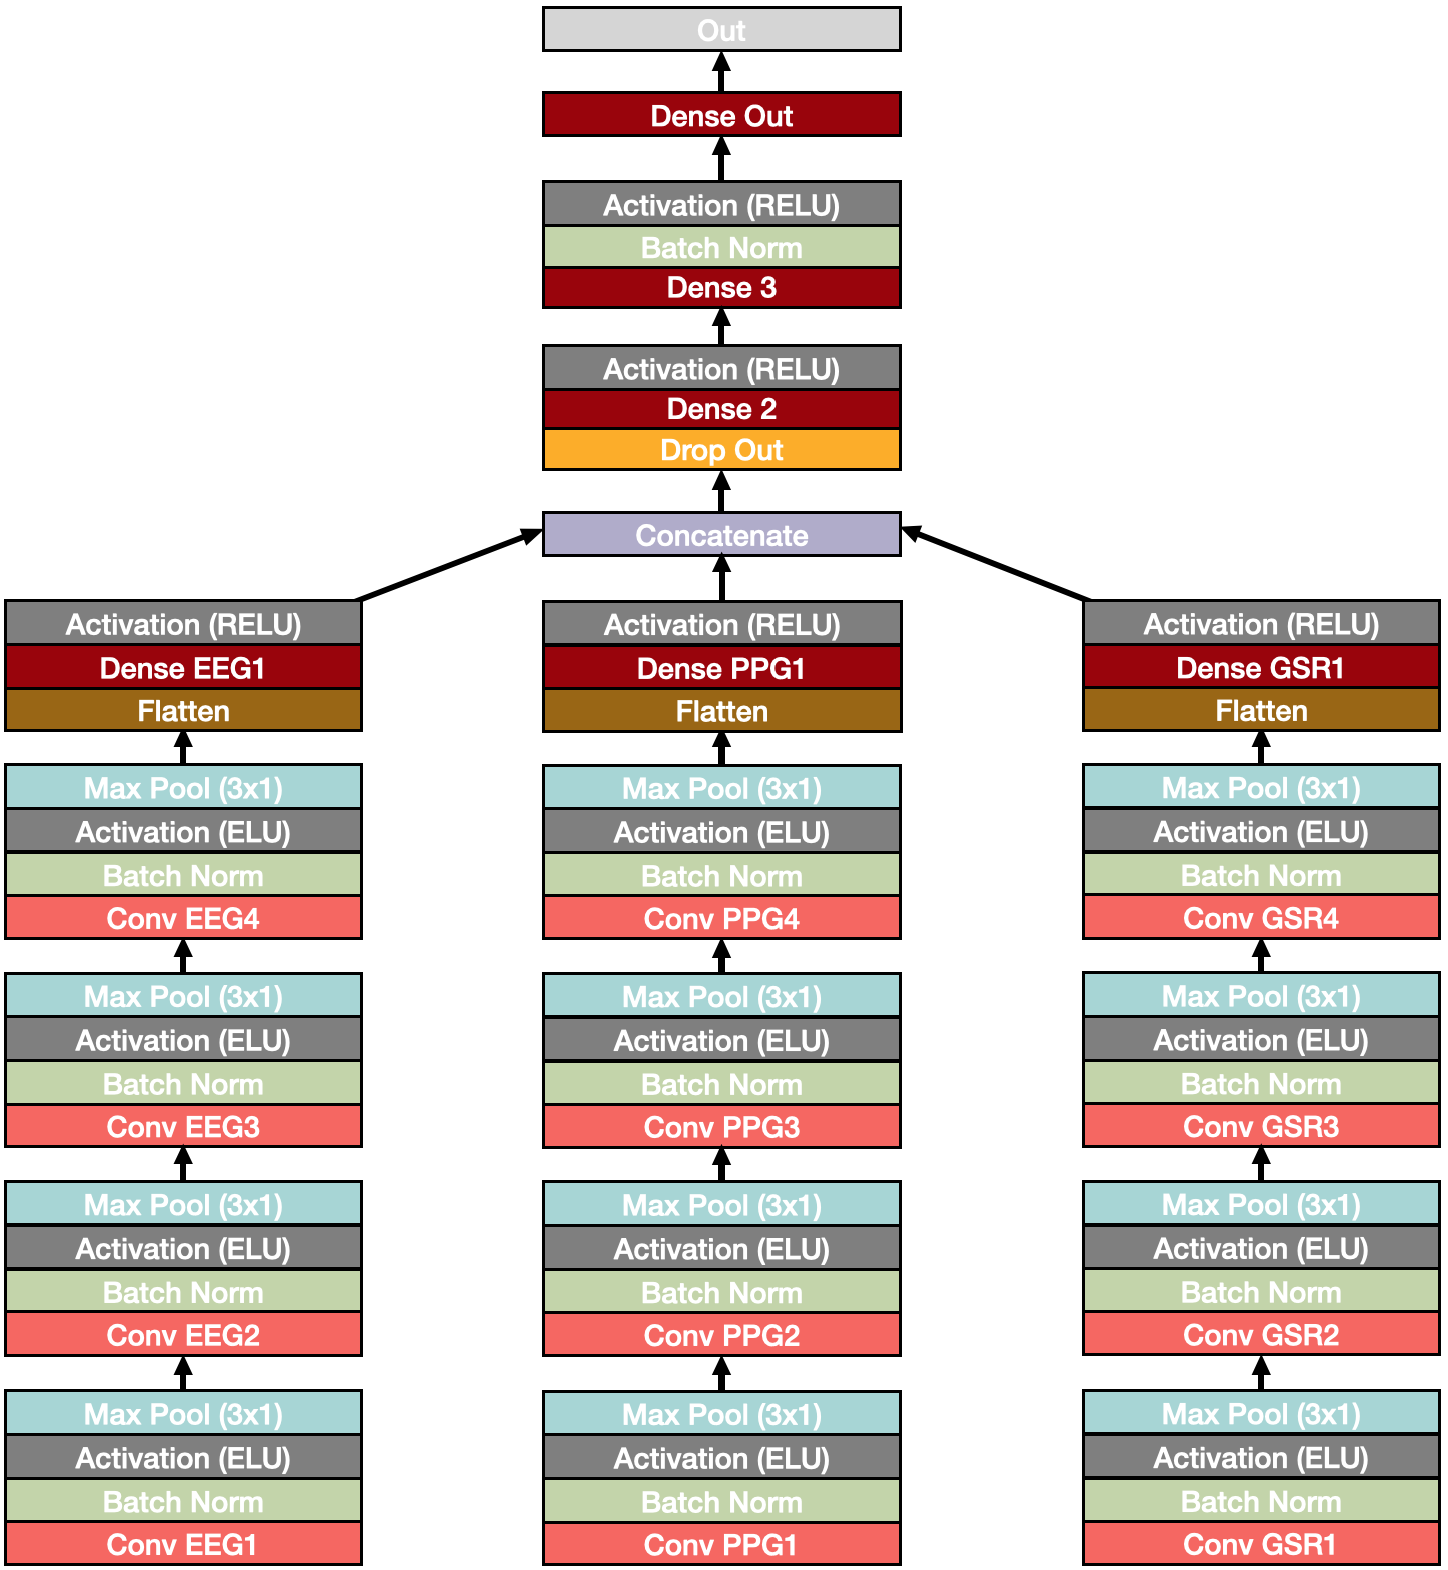
\includegraphics[scale=0.50]{multi_model_architecture}
\caption{Multimodal network architecture. The network constitutes a convolutional part of four convolutional blocks for each of three subparts. All three distinct parts were flattened and concatenated. The prediction part of the network constitutes several dense layers.}\label{fig:multiarchitecture}
\end{figure}

\subsection{Network Performance Evaluation}
As the reader might recall from Section \ref{section:DNN} we opted for individually tailored DNN's, trained for each respondent separately. Hence, for each of the the four contrasted architectures, the predictions of all personally trained network were aggregated, after which performance was assessed by means of the following three performance metrics. 

The Mean Absolute Error, hereafter referred to as "MAE",  is the first utilized performance metric, defined as:

$$\frac{1}{n} \sum^n_{i=1}|f(x_i)-y_i|$$
where $n$ refers to the total amount of testing windows, $f(x_i)$ to the predicted value for window $i$ and $y_i$ to the true label of window $i$.
The MAE constitutes the most straightforward metric for DNN performance assessment, for its value can simply be interpreted as the average misprediction. 

The Root Mean Squared Error, hereafter referred to as "RMSE", is the second utilized performance metric, defined as:

$$\sqrt{{\frac{1}{n} \sum^n_{i=1} \Big( f(x_i)-y_i} \Big) ^2}$$
where $n$ refers to the amount of testing windows, $f(x_i)$ to the predicted value for window $i$ and $y_i$ to the true label of window $i$. The RMSE is closely related to the MAE, differing in that it tends to punish big differences more severely. 

Finally, Pearson's correlation coefficient, hereafter referred to as simply "correlation", constitutes the third utilized performance metric, defined as:

$$r_{X,Y} = \frac{cov(X,Y)}{\sigma_{X} \sigma_{Y}}$$
where $X$ refers to the predicted test windows,  $Y$ to the true labels of the test windows, $cov(X,Y)$ to their covariance and $\sigma_{X}$ and $\sigma_{Y}$ to the standard deviation of $x$ and $y$ respectively.  Conceptually, correlation can be interpreted as the strength of the linear relationship between predictions and their labels, thus providing an indication of network performance. 

\vspace{8mm}
\section{Results}
Before addressing network performance, we firstly present a description of all window labels as depicted in Figure \ref{fig:labels}. Displayed is an aggregation of the window labels of all participants, resulting in a total of 9474. It is immediately noticeable that the distribution displays a right-skewed tendency, with a median of 0.29 and an 90\% upper-bound quantile of 0.64. This demonstrates that there is a considerable underrepresentation of high workload windows in our data, the implication of which will be addressed in a subsequent section. 

\vspace{3mm}
\begin{figure}[h]
\centering
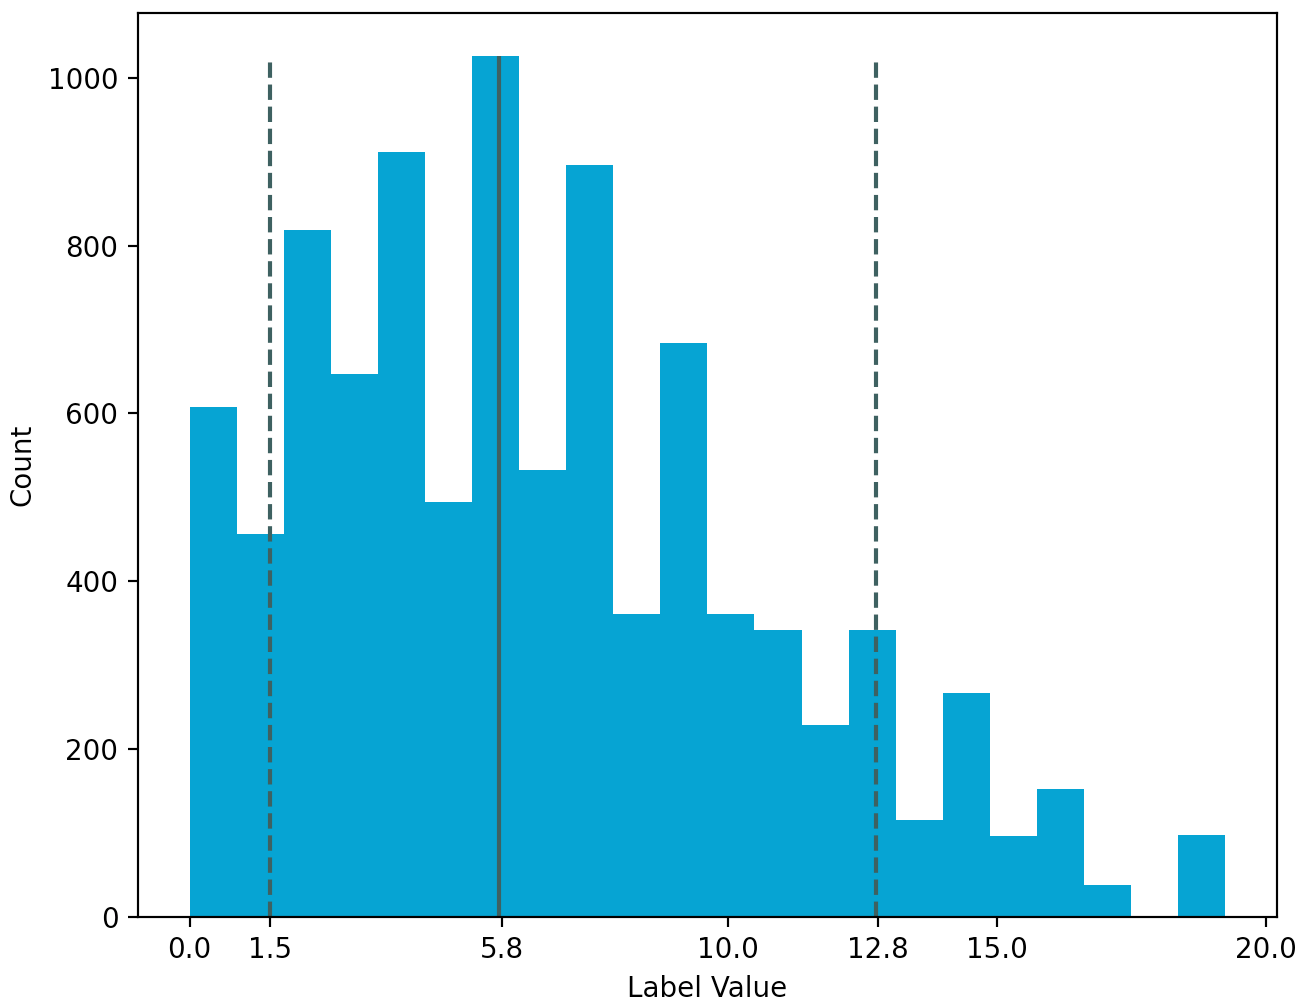
\includegraphics[scale=0.5]{labels.png}
\caption{Distribution of the aggregate of all window labels. The solid line represents the median, whereas the two dashed lines represent the 10\% and 90\% quantiles respectively. }\label{fig:labels}
\end{figure}

\subsection{Results: Performance Metrics}
Depicted in Table \ref{table:results} are the performance metrics of all four network architectures. Most striking is the performance of the multimodal architecture, scoring consistently worse across all metrics when compared with the unimodal EEG and GSR architectures.

Performance in terms of MAE is most favorable for the EEG architecture, closely followed by the GSR architecture. The multimodal architecture performs worse than the aforementioned, ultimately followed by the PPG architecture, which scored worst in terms of MAE. Results in terms of RMSE adheres to a similar pattern, which is not surprising, given that the RMSE and MAE are closely related. RMSE values are consistently higher as compared with MAE, which can be attributed to the tendency of the RMSE to punish strong deviations more severely. The correlation between predictions and labels are indicative of a similar pattern, in which the EEG architecture scores best, followed by the GSR, multimodal and PPG architectures respectively. Despite the consistency in this pattern, an interesting disparity is that the differences in terms of correlation across the four architectures are more substantial. In addition to the aforementioned results, we also assess network performance on the training data, with which we attempt to gain insight into the potential occurrence of overfitting. Table \ref{table:appendix} in Appendix \ref{sec:appendix} presents the performance of the four network architectures, but now employed on the training data.  It becomes apparent that the unimodal architectures perform better by a substantial margin on the training data: both MAE and RMSE values are considerably lower, whereas the correlation between predictions and labels are considerably higher. This is indicative of rather substantial overfitting. This tendency, although much less profound, is also observable for the multimodal architecture.

\vspace{7mm}
\bgroup
\def\arraystretch{1.4}  
\begin{table}[h]
\begin{center}
\caption{Deep Neural Network Performance Metrics} \label{table:results}
\begin{tabular}{lllll}
\hline
 &
  \begin{tabular}[c]{@{}l@{}}MAE (sd) \\ 0-1 scale\end{tabular} &
  \begin{tabular}[c]{@{}l@{}}MAE (sd) \\ 0-20 scale\end{tabular} &
  \begin{tabular}[c]{@{}l@{}}RMSE \\ 0-1 Scale\end{tabular} &
  \begin{tabular}[c]{@{}l@{}}Pearson's\\ Correlation\end{tabular} \\ \hline
EEG        & 0.110 \,\,(0.15) & \,\,2.206 \,\,(3.08) & \,\,0.154 & 0.688 \\
PPG        & 0.136 \,\,0.18) & \,\,2.717 \,\,(3.59) & \,\,0.180 & 0.530 \\
GSR        & 0.119 \,\,(0.16) & \,\,2.377 \,\,3.18) & \,\,0.159 & 0.653 \\
Multimodal & 0.128 \,\,(0.17) & \,\,2.570 \,\,(3.33) & \,\,0.167 & 0.609 \\ \hline
\end{tabular}
\end{center}
\raggedright{ \emph{\newline Values between parentheses are standard deviations. MAE refers to Mean Average Error. RMSE refers to Root Mean Square Error. }}
\end{table}
\vspace{7mm}

In order to formally contrast performance across various network architectures (as employed on the training data), we conduct several independent sample t-tests, with which we test differences in absolute (window) prediction error. The absolute prediction error is the same as mean absolute error (MAE), except for that it is not averaged per architecture. Testing is done two-sided with $\alpha = 0.05$. The average absolute prediction error per architecture (i.e. MAE) is not repeated alongside the statistical tests, for they are already displayed in Table \ref{table:results}. Absolute prediction errors of the unimodel EEG architecture were found to be significantly lower as compared with those of the multimodel architecture $t(1936)=-2.566, p=0.01$. No significant difference in terms of absolute prediction error between the EEG and GSR architectures were found $t(1936)=-1.188, p=0.24$, and equally so, no significant differences between the GSR and multimodal architectures were found $t(1936)=-1.463, p = 0.144$. Lastly, absolute prediction errors of the GSR architecture were found to be significantly lower as compared with the PPG architecture $t(1936)=-2.636 , p = 0.008$, but no significant differences between the GSR and multimodal architecture were found $t(1936)=-1.164 , p = 0.245$.

\subsection{Results: Further Exploration}
To further explore the differences in performance, a graphical visualization of the distribution of window prediction errors per architecture are depicted in Figure \ref{fig:mae_hist}.

\vspace{7mm}
\begin{figure}[h]
\centering
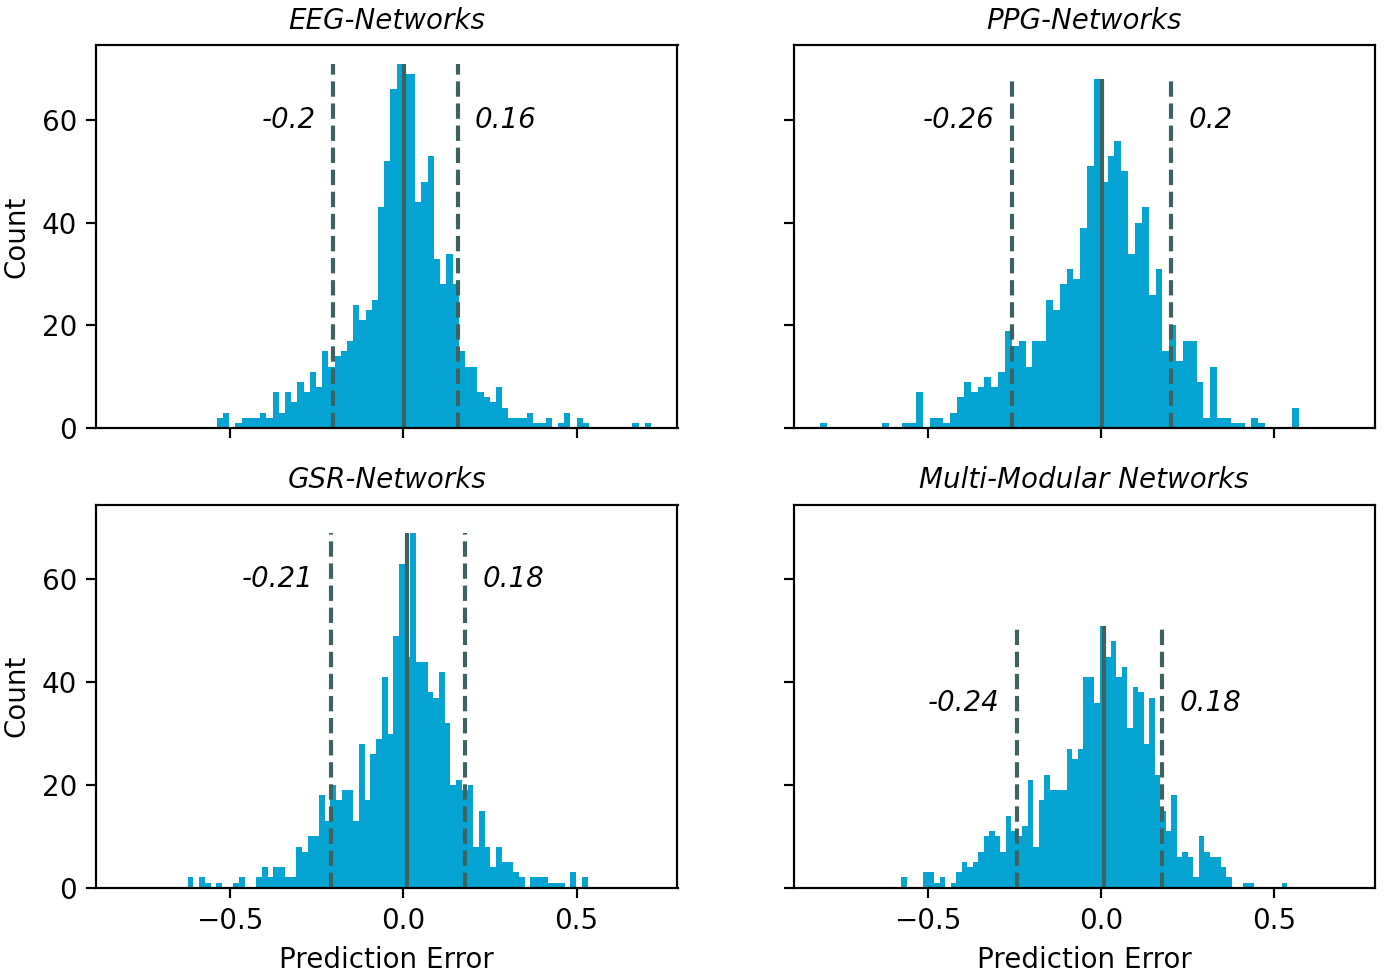
\includegraphics[scale=0.56]{error_hist.png}
\vspace{2mm}
\caption{Distribution of window prediction error per network architecture. The solid lines represent the median, whereas the dashed lines represent the 10\% and 90\% quantiles respectively. } \label{fig:mae_hist}
\end{figure}
\vspace{4mm}

In line with the previously discussed performance metrics, it becomes readily apparent that the distribution of the prediction errors for the architecture that scored best across all metrics, i.e. the EEG architecture, approximates the most narrowly shaped normal distribution. This may be derived by the strong accumulation around the zero error mark (i.e. visually "peaked") and the relatively flat tails. The two worst performing architectures, i.e. the multimodal and PPG architectures, display relatively thick tails, and are observed to have less strong accumulation around the 0 error mark (i.e. visually "less-peaked"). This is equally so demonstrated by the 10\% and 90\% quantiles, residing farthest from the median.  All distributions are observed to be slightly left-skewed, as indicated firstly by shape and secondly by the fact that 10\% quantiles are farther removed from zero as compared with the 90\% quantiles. Despite that this left-leaning tendency is observable for all network architectures, it is most profound for the PPG and multimodal architectures. 

We further explore our results by means of a graphical visualization of absolute (window) prediction error contrasted against window label value. This relationship is depicted in Figure \ref{fig:mae_scatter}.

\begin{figure}[h]
\centering
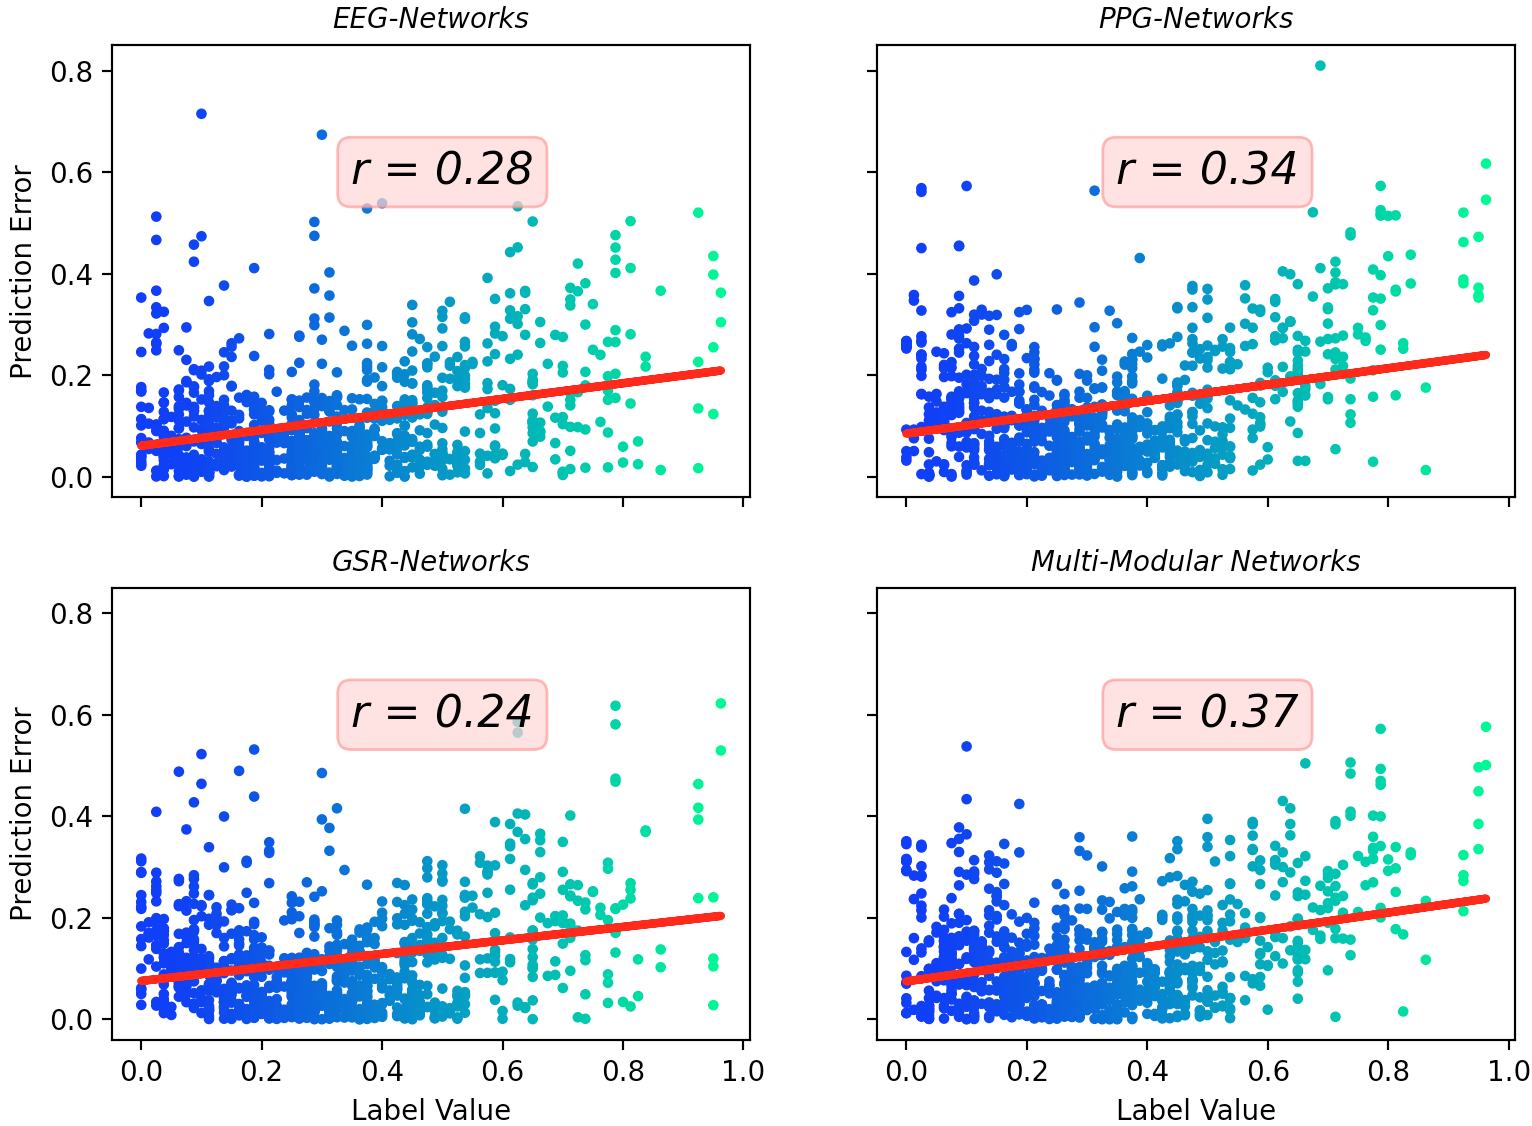
\includegraphics[scale=0.5]{mae_scatter.png}
\caption{Relationship between absolute window prediction error and window label value. The lines represent the linear relationships between absolute prediction errors and label values. The values \textit{r} represent the Pearson's correlation coefficients as captured by the lines.} \label{fig:mae_scatter}
\end{figure}
\vspace{7mm}

\newpage
It becomes apparent from Figure \ref{fig:mae_scatter}}, that higher labeled windows are substantially less prevailing, as indicated by the thin spreading of dots at the right hand side of the plots. This is conform to the conclusion drawn from the earlier depicted Figure \ref{fig:labels}. Most noteworthy is that for all architectures, a moderately high linear relationship between absolute window prediction error and the respective label size can be observed. This is indicated by both the moderately ascending slopes, and the moderately high (and positive) correlation coefficients $r$. Substantively, this implies that all network architectures are considerably less accurate when predicting high labeled windows. This tendency is strongest for the multimodal architecture. For both the EEG and GSR architectures, this linear relationship is observed to be weaker, although still of a noteworthy magnitude.
\vspace{5mm}

\section{Discussion \& Conclusion}
The unimodal EEG architecture was found to consistently perform best across all performance metrics. The second best performance was attained by the unimodal GSR architecture, followed by the multimodal architecture, and lastly, the unimodal PPG architecture. For various pairs of architectures, we formally tested differences in terms of their absolute prediction errors. Statistical evidence indicated that the unimodal EEG architecture significantly outperformed the multimodel architecture. In addition, we presented statistical evidence indicating that both the unimodal EEG and unimodal GSR architectures, outperformed the unimodal PPG architecture. In order to explore the extent to which our networks suffered from overfitting, we applied them towards the training data. These results demonstrated rather substantial overfitting, particularly so for the three unimodal architectures. Lastly, we illustrated the linear relationship between absolute window prediction errors and label sizes. This relationship was found to be moderately high across all architectures, indicating that they performed worse in predicting higher labeled windows. This tendency was found to be strongest for the two worst performing architectures, i.e. the multimodal and unimodal PPG architectures. 

\subsection{Discussion}
Out of all three unimodal architectures, the EEG architecture was found to perform best. The EEG modality may thus be considered the most adequate predictor of workload. This confirms the first expectation we posed in the introduction, and is conform to previous research by \cite{hogervorst2014combining}. In addition to this, perhaps the most noteworthy result is that the multimodal architecture was outperformed by the unimodal EEG architecture. As posed in the introduction, we hypothesized the contrary. This expecation was partly based on a number of preceding studies, which consistently found a multimodal architecture to perform superiourly \cite{dolmans2020perceived, han2020classification, rastgoo2019automatic, yin2017recognition}. In the subsequent section we aim to rationalize this result. 

Part of the reason could be the network architecture. Conform to  \citeA{han2020classification}, a shallow head network architecture was adopted, solely consisting of several fully connected dense layers. However, as was reported upon in Section \ref{sec:related}, some other studies opted for a fundamentally different design philosophy \cite{dolmans2020perceived, rastgoo2019automatic}. Further investigation into alternative head network architectures could have resulted in a more adequately performing network,  but would have increased the computational expenses considerably. Besides this, an important consideration is the oftentimes precarious balance between model complexity and simplicity. A model that is overly complex is in increased peril of overfitting, i.e. performing well on training data, but failing to generalize to testing data \cite{lever2016points}. Overfitting can especially be anticipated when training a relatively complex DNN on a small amount of data \cite{aggarwal2018neural, feng2019using}. As was expounded upon in Section \ref{section:DNN}, we opted for personally trained networks. A consequence of this is that we trained on small amounts of data. Indeed, strong evidence in favor of overfitting was found for the unimodal architectures, indicating that these networks were too complex to be trained on such small amounts of data. Surprisingly, the even more complex multiodal architecture only displayed minor overfitting. Despite this, it should be acknowledged that the core of the multimodal architecture is a composite of the, apparently overly complex, unimodal architectures, which most likely contributed to its relatively inadequate performance. These insights are distilled into various future research recommendations, presented in the later Section \ref{sec:future}.

Another noteworthy result was the illustrated linear relationship between absolute prediction errors and their respective label scores (as visualized in Figure \ref{fig:mae_scatter}). It was demonstrated that all four architectures were consistently less accurate in predicting high labeled windows.  A credible explanation for this is the relatively minor presence of high labeled windows in our data (as visualized in Figure \ref{fig:labels}). Naturally, when a relatively small amount of high labeled windows are present in the training set, a DNN is unable to adequately learn to predict such windows. Again, various strategies to handle this are proposed in Section \ref{sec:future}. 

Finally, despite that several comparisons of absolute prediction errors across architectures were found to be statistically significant, all differences in terms of MAE and RMSE were rather small absolutely speaking. The statistical significance of several of the conducted t-tests may particularly be attributed to the vast amount of degrees of freedom with which was tested. We therefore recognize that the performance of most of our architectures were rather close, and reflect on the following: in opposite to our finding, suppose that a multimodal approach would have lead to a small improvement in performance over the unimodal approaches. Would this justify the addition in complexity,  the considerable increment in computational expenditure and the necessity to invest in a multitude of different physiological sensors? In other words, isn't the already adequately performing, and much less complex unimodal EEG approach sufficient for most tasks at hand? The answer to these questions is heavily dependent upon context.

\subsection{Limitations \& Future Research Recommendations} \label{sec:future}
Additional research is necessary to gain insight into optimally performing network architectures for small data scenario's such as the current.  More specifically,  further insights are required into 1) which network architectures are able to minimize overfitting and 2) which network architecture is most suitable for a multimodal approach. An effective technique with which this can be investigated is HPO, since apart from optimizing hyperparamaters, a network architecture in its entirety can be optimized. Thus, a recommendation for future research is to gain more insight into which type of DNN architectures are suitable for small dataset scenarios.

As became apparent, all architectures were found to be less precise in predicting high labeled windows, attributable to the fact that such windows were relatively uncommon in our data. In theory, the absence of high labeled windows could result from two factors. Firstly, participants could have refrained from reporting high workload on the NASA-TLX items that were utilized for labeling. Alternative labeling approaches may be compared in order to address this. Ideally, one would want to contrast various labeling strategies, such that the best performing can be adopted. Examples of alternatives labeling approaches are a standardized version of the NASA-TLX, or an objective difficulty score for each task, as was proposed by \citeA{dolmans2020perceived}. Secondly, it might be that participants simply did not experience high workload throughout the experiment. The may be addressed by designing the experiment such high workload tasks are prevalent. Pretesting might help to ensure this.

Finally, as was discussed before, the personal differences that are inherent to physiological data were acknowledged by using individually trained networks. However apart from such between-personal differences, physiological data might be characterized by between-occasional differences as well. To give an example, PPG measurement is dependent upon various occasional factors, such as amongst others the amount of emitted surrounding light, body position, cardiovascular stresses, etc. \cite{lemay2014application}. Even for the same person, these contextual factors may differ across occasions, potentially endangering the generalizability of the trained networks. Further research is necessary in order to determine the robustness of personally trained networks at different occasions.

\subsection{Conclusion}
The current research adds to the body of knowledge on deep learning based workload assessment. We contrasted various approaches to workload prediction by means of several physiological sensors. Four network architectures were contrasted in performance, including a unimodal EEG architecture, a unimodal GSR architecture, a unimodal PPG architecture and a multimodal architecture.  In the introduction we posed two key research goals. Firstly, with this research we sought to explore which modality constitutes the most adequate predictor of workload. This was expected to be the EEG modality. Altough all modalities were found to perform rather satisfactory, we conclude that indeed the EEG modality constitutes the most adequate predictor of workload (opposed to PPG and GSR). Secondly, with this research we sought to determine whether a multimodal network architecture was preferable over three simpler unimodal architectures. Based on our results a multimodal approach was unjustified, however several explanations were considered that could potentially refute this finding. Further research is therefore necessary. This future research will ideally investigate upon 1) network architectures that prevent substantial overfitting in a small dataset scenario,  2) an appropriate architecture for a multimodal approach in a small dataset scenario, 3) the feasibility of different labeling strategies and 4) the extent to which personally trained networks can be generalized towards different occasions.

\newpage
\bibliographystyle{apacite}
\bibliography{References}

\newpage
\appendix
\section{Appendix} \label{sec:appendix}
\subsection*{Performance on Training Data}
\setcounter{table}{0}    
\counterwithin{table}{section}

\vspace{15mm}
\bgroup
\def\arraystretch{1.6}%  
\begin{table}[h]
\begin{center}
\caption{Deep neural network performance metrics on training data}
\label{table:appendix}
\begin{tabular}{lllll}
\hline
 &
  \begin{tabular}[c]{@{}l@{}}MAE (sd) \\ 0-1 scale\end{tabular} &
  \begin{tabular}[c]{@{}l@{}}MAE (sd) \\ 0-20 scale\end{tabular} &
  \begin{tabular}[c]{@{}l@{}}RMSE (sd) \\ 0-1 Scale\end{tabular} &
  Correlation \\ \hline
EEG        & 0.038 \,\,(0.06) & \,\,0.761 \,\,(1.14) & \,\,0.070 & 0.944 \\
PPG        & 0.077 \,\,(0.11) & \,\,1.541 \,\,(2.28) & \,\,0.114 & 0.838 \\
GSR        & 0.085 \,\,(0.12) & \,\,1.700 \,\,(2.43) & \,\,0.122 & 0.813 \\
Multimodal & 0.116 \,\,(0.16) & \,\,2.331 \,\,(3.11) & \,\,0.156 & 0.670 \\ \hline
\end{tabular}
\end{center}
{\raggedright \emph{ \newline Values between parentheses are standard deviations. Mae refers to Mean Average Error. RMSE refers to Root Mean Square Error. } \par}
\end{table}
\vspace{3mm}

\end{document}
